%!TEX root =  ../main.tex


\subsection{Derivatives of Exponentials}


\objective{Describe and use the special status of $e^x$ amongst exponential equations}


As we move past power function, derivatives become a lot harder to compute.  If we
begin with the premise that there is some exponential function which is its own 
derivative --- that the height of the function at every point is the same as its slope
--- then we should find constant for the base.  Empirically, it is easy to see that
such a number is between 2 and 3, but how can we be more precise?  We
begin with the definition
$$
f'(x) = \lim_{h\rightarrow0}\frac{f(x+h)-f(x)}{h}
$$
We will use the letter $e$ next, but assume we do not know its exact value.  In
the problem set, you saw that it's definition is
$$
e = \lim_{h\rightarrow\infty}\left(1+\frac{1}{h}\right)^h
$$
and so right away we see we are dealing with opposite limits.  We can convert
from a limit at infinity to a limit at zero by taking the reciprocal of the variable
at every instance.  This leads to a modified definition of $e$:
$$
e = \lim_{h\rightarrow0}\left(1+\cfrac{1}{\frac{1}{h}}\right)^{\frac{1}{h}}
$$
Armed wth compatible limits, let us return to the definition of a derivative.
$$
(e^x)'  = \lim_{h\rightarrow0}\frac{e^{x+h}-e^x}{h}
$$
By the properties of exponents, a sum in the degree must come
from a multiplication of the bases (i.e. $e^{x+h}=e^x\cdot{}e^h$).
Factoring out $e^x$, we get
$$
(e^x)' = e^x \cdot{}\lim_{h\rightarrow0}\frac{e^h-1}{h}
$$
Will our definition of $e$ work here?  Substituting it in is very messy, but cleans up
perfectly.  Just evaluating the limit,
\begin{align*}
	\lim_{h\rightarrow0} & \frac{\left[\left(1+\cfrac{1}{\frac{1}{h}}\right)^{\frac{1}{h}}\right]-1}{h} &\\
	& \frac{1+\left(\cfrac{1}{\frac{1}{\frac{1}{h}}}\right) - 1}{h} &\\
	& \frac{\cfrac{1}{\frac{1}{h}}}{h} & \Rightarrow \frac{h}{h} \\
	& = 1
\end{align*}

\begin{derivation}{Derivative of $e^x$}
$$
(e^x)' = e^x
$$
\end{derivation}

\personfeature[0in]{\chapdir/pics/Charles_Hermite_circa_1901_edit}{Charles Hermite}{1822
- 1901}{was a French mathematician who did research on number theory, 
quadratic forms, invariant theory, orthogonal polynomials, elliptic functions, and algebra.
He was the first to prove that $e$, the base of natural logarithms, is a transcendental number. 
His methods were later used by Ferdinand von Lindemann to prove that $\pi$ is transcendental.
\href{https://en.wikipedia.org/wiki/Charles_Hermite}{Wikipedia}}

\subsection{Implications}
How does this explain the behavior of $2^x, 3^x$ or any other base?  The limit portion of
the work shown above was equal to 1, but if we had substituted any other number in,
we would have obtained some constant.  We can extend the definition of exponential
derivative like so:

\begin{derivation}{Derivative of $b^x$}
$$
(b^x)' = b^x \cdot{} \ln{b}
$$
\end{derivation}

Often we will need to apply the Chain Rule, since the exponent is rarely just $x$
$$
\left(e^{f(x)}\right)' = e^{f(x)} \cdot f'(x)
$$

Lastly, if $e^x$ is it's own derivative, then it is its own anti-derivative as well:
$$
\int e^xdx = e^x + C
$$

The TI-8* has an $e^x$ function (2nd-LN) and most computer programs (e.g. MS Excel)
have a function \texttt{exp()}, which is the same thing.

\begin{figure}
\begin{centering}
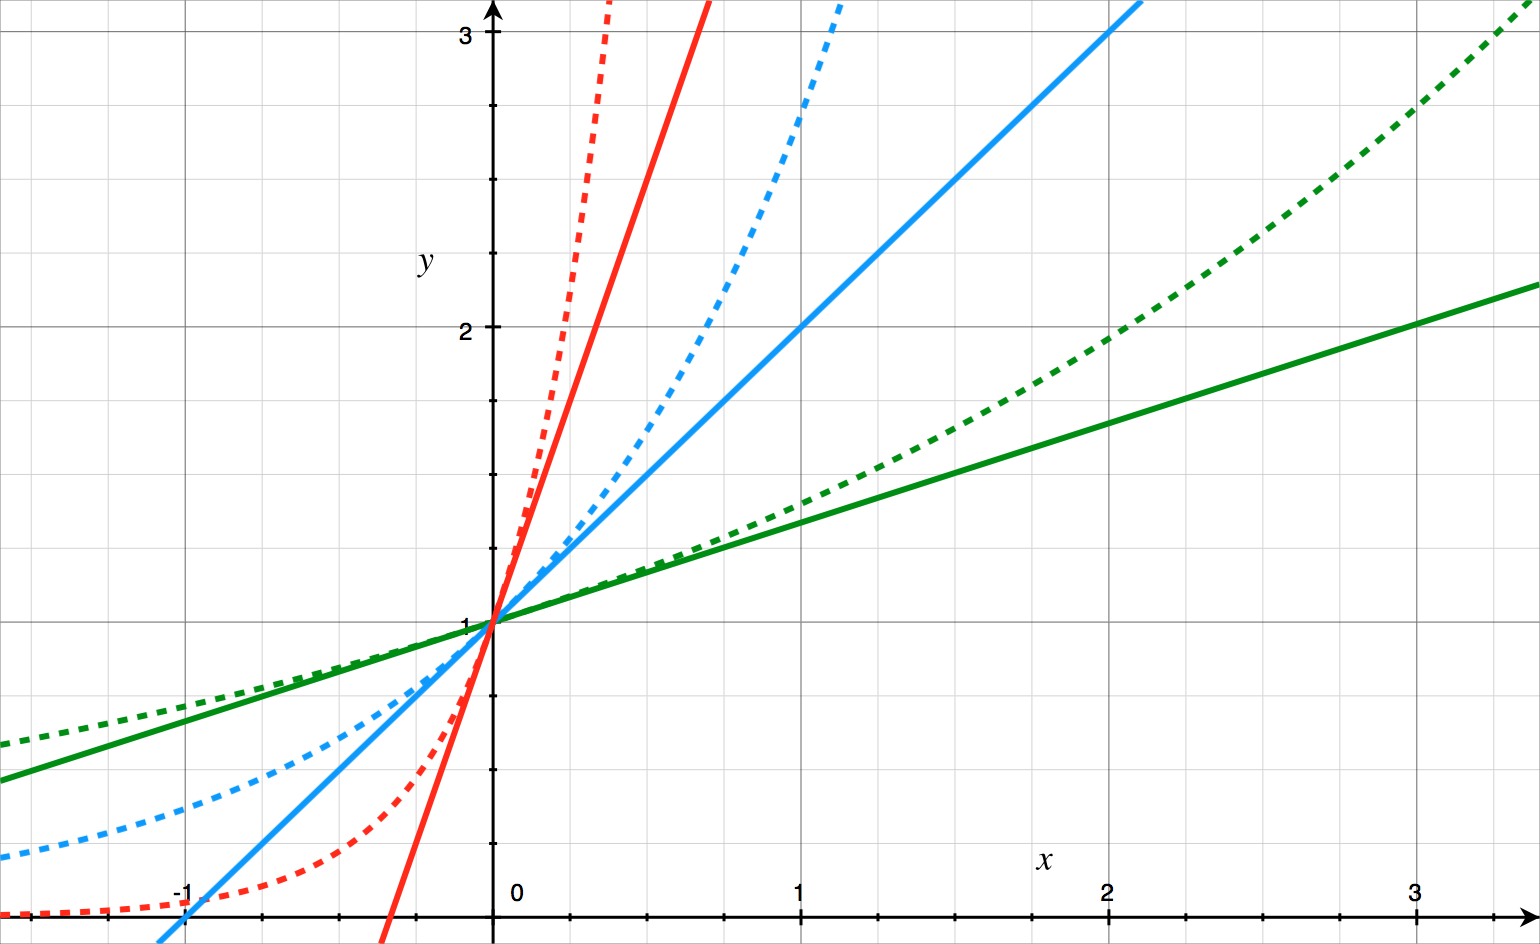
\includegraphics[width=\textwidth]{\chapdir/pics/exponentialderivatives}
\caption[Exponential tangent lines at (0,1)]{A set of exponential equations tangent lines at (0,1), with original function dotted.  $1.4^x$ in green, $e^x$ in blue, $20^x$ in red.}
\end{centering}
\end{figure}